\documentclass[a4paper,10pt]{article}

\usepackage{graphicx}
\usepackage[spanish, activeacute]{babel}
%opening
\title{Sintesis de Deadlock}
%\subtitle{Capitulo 6 SilverChair}
\author{El grupete}

\begin{document}

\maketitle


\section{Deadlock}

\subsection{Introducci'on}
En un entorno de multiprogramaci'on varios procesos pueden competir por un numero finito de recursos. Un procesos solicita recursos y si estos no estan disponibles, el proceso queda en estado de espera. Puede pasar que los procesos en espera nunca cambien de estado porque los recursos que necesitan los tienen otros procesos que tambien est'an en espera, a esta situaci'on se la llama Dreadlock.

\subsection{Modelo del sistema}
Los recursos se dividen en varios tipos, cada uno de los cuales consiste en ejemplares id'enticos. 
En el modo de operaci'on normal, un proceso solo puede utilizar un recurso en la secuencia siguiente:
\begin{itemize}
 \item Solicitud: Si la solicitud no se puede atender de inmediato entonces el proceso solicitante debe esperar a que pueda adquirir el recurso.
 \item Utilizaci'on
 \item Liberaci'on
\end{itemize}
La solicitud y liberaci'on de recursos son llamadas al sistema, estas pueden lograrse a travez de las operaci'on wait y signal sobre sem'aforos.
Una tabla del sistema registra si cada uno de los recursos esta libre o asignado, y si esta asignado a que proceso. Si un proceso solicita un recurso que ya esta asigando entoces lo puede encolar en la cola de espera de ese proceso.
Un conjunto de procesos se encuentra en Deadlock si cada uno espera un suceso que solo puede originar otro proceso del mismo conjunto.

\subsection{Caracterizaci'on de los bloqueos mutuos}
\subsubsection{Condiciones necesarias}
Una situacion de deadlock puede surgir si y solo si en un sistema se presentan las siguientes cuatro condiciones:
\begin{itemize}
 \item Exclusion mutua: Por lo menos un recurso debe reternerse en modo no compartido; es decir, solo un proceso puede usar el recurso a la vez. Si otro proceso solicita el recurso debera esperar a que sea liberado.
 \item Retenci'on y espera: debe haber por lo menos un proceso que retenga un recurso y espere adquirir otros recursos retenidos por otros procesos.
 \item No apropiaci'on: Los recursos no se pueden quitar. Es decir, un recurso solo puede ser liberado por el proceso que lo tiene despues de haber cumplido su tarea.
 \item Espera circular: Debe haber un conjunto ${P0,...,Pn}$ de procesos en espera, tales que $P0$ espera un recurso retenido por $P1$, $P1$ espera un recurso retenido por $P2$,..., $Pn-1$ espera un recurso retenido por $Pn$ y $Pn$ espera un recurso retenido por $P0$.
\end{itemize}
La condici'on de espera circular implica la de retenci'on y espera, sin embargo es util verlas por separado.

\subsubsection{Grafo de asignaci'on de recursos}
Es un grafo dirigido donde los nodos son procesos o recursos. Una arista de un recurso a un proceso indica que ese recurso esta siendo utilizado por ese proceso (arista de asignaci'on). Una arista de un proceso a un recurso indica que ese proceso solicito ese recurso (arista de solicitud).
A los procesos los dibujamos con redondeles y a los recursos con cajitas. Como pueden haber muchas instancias de un mismo tipo de recurso en las cajitas dibujamos puntitos que representan cuantas instancias de ese recurso hay. Ejemplo: si tenemos dos impresoras dibujaremos una cajita con dos puntos dentro, en este caso podr'an salir dos flechas de este nodo (una por impresora). 
IMPORTANTE: Si el grafo no contiene ciclos entonces ningun proceso esta en deadlock, por otra parte, si hay ciclo entonces PUEDE haber un deadlock.
Si cada tipo de recurso tiene un solo ejemplar, entonces un ciclo representa que ha ocurrido un bloqueo mutuo y todos los procesos en el ciclo estan en deadlock.
Si el ciclo comprende solo un conjunto de tipos de recursos, cada uno con un solo ejemplar, entonces ha ocurrido un bloqueo mutuo entre todos los procesos en el ciclo.

\subsubsection{M'etodos para manejar Deadlocks}
Existen dos m'etodos principales para tratar el tema del deadlock. Podemos usar un protocolo para que el sistema nunca entre en deadlock o podemos permitir que entre y se recupere.
Primero consideraremos m'etodos para que el sistema nunca entre en deadlock. Para ello contamos con dos m'etodos comunes: la prevenci'on y la evitaci'on.

\subsection{Prevenci'on de bloqueos mutuos}
Para que haya deadlock deben presentarse cada una de las cuatro condiciones necesarias. Veremos distintas maneras de evitar cada una de estas condiciones, previniendo el deadlock.

\subsubsection{Exclusi'on Mutua}
Los recursos compartibles no pueden participar en un deadlock.
Por lo general no es posible evitar el deadlock negando la condici'on de exclusi'on mutua. Por su propia condici'on algunos recursos no son compartibles.

\subsubsection{Retenci'on y espera}
Para asegurar que la condici'on de retenci'on y espera nunca se de, debemos garantizar que cuando un proceso solicita un recurso, no retenga otros.
\begin{itemize}
 \item Un protocolo que puede usarse es que cada proceso solicite todos los recursos antes de empezar su ejecuci'on.
 \item Otro similar es que un proceso solo pueda pedir recursos si no tiene ninguno asignado. Si necesita m'as recursos que los que tiene en un momento dado, debe liberar todo para volver a pedir lo que necesita.
\end{itemize} 
La desventaja de estas pol'iticas es que puede pasar que se pidan recursos que nunca ser'an usados por el proceso que los solicito.
Adem'as es posible un bloqueo indefinido, si un proceso pide varios recursos populares, es posible que nunca le sean adjudicados porque estan en uso por otros procesos (es una especie de inanici'on, pero el libro no lo nombra asi).

\subsubsection{No apropiaci'on}
La tercer condicion es que no haya apropiaci'on de recursos: para evitar esto podemos permitir la apropiac'ion ;P
\begin{itemize}
 \item Si un proceso que tiene un recurso solicita otro que no se le puede dar de inmediato, entonces se le sacan todos los recursos que tiene y volver'a a ejecutar cuando se le puedan asignar todos los recursos que pidi'o mas los que ten'ia.
 \item Si un proceso solicita recursos que no estan disponibles comprobamos si estan asignados a otro proceso que espera mas recursos, en cuyo caso expropiamos los recursos deseados del proceso en espera y los asignamos al proceso solicitante. Si los recursos no est'an disponibles ni asignados a un proceso en espera, el proceso debera esperar.
\end{itemize}
Este protocolo se usa cuando se puede guardar con facilidad el estado de los recursos, como CPU y memoria principal. Es un garron para impresora o cintas.

\subsubsection{Espera circular}
Una forma de asegurar que no se presente la condici'on de espera circular es imponer una ordenaci'on total de todos los tipos de recursos y requerir que cada proceso solicite los recursos en orden ascendente.

\subsection{Evitaci'on de bloqueos mutuos}
Otro m'etodo para evitar los bloqueos mutuos consiste en requerir informaci'on adicional sobre como se solicitar'an los recursos. Cada solicitud requiere que el sistema considere los recursos disponibles en ese momento, los actualmente asignados a cada proceso, y las futuras solicitudes y liberaciones de cada proceso, para decidir si puede satisfacer la solicitud presente o debe esperar para evitar un posible deadlock futuro.
Los diversos algoritmos difieren en la cantidad y tipo de informaci'on que requieren. El modelo mas sencillo y 'util requiere que el proceso declare la cantidad m'axima de recursos que usar'a para cada tipo de recurso. Un algoritmo de evitacion de deadlock examina din'amicamente el estado de asignaci'on de recursos para asegurar que no pueda presentar una condici'on de espera circular. El estado de asignaci'on de recursos viene definido por el n'umero de recursos disponibles y asignados, y por la demanda m'axima de los procesos. Un estado es seguro si el sistema puede asignar recursos a cada proceso (hasta el m'aximo) siguiendo algun orden y aun asi avitar el deadlock. Mas formalmente un sistema se encuentra en estado seguro s'olo si existe una secuencia segura. Una secuencia de procesos $P_{1},..,P_{n}$ es segura para el estado actual de asignaciones si, para cada $P_{i}$, los recursos que aun puede solicitar $P_{i}$ pueden satisfacerse con los recursos actualmente disponibles mas los retenidos por todos los $P_{j}$, donde $j<i$. En esta situaci'on si los recursos que necesita $P_{i}$ no estan inmediatamente disponibles, entonces $P_{i}$ puede esperar a que terminen todos los procesos $P_{j}$. Una vez terminados, $P_{i}$ puede obtener todos los recursos necesarios, completar la tarea, devolver los recursos que se le han asignado y terminar. Cuando $P_{i}$ termina, $P_{i+1}$ puede obtener todos los recursos necesarios, etc. Si no existe esta secuencia, se dice que el estado es $inseguro$.
Un estado seguro NO ES un estado de bloqueo mutuo, y un estado de bloqueo mutuo ES un estado inseguro, pero no todos los estados inseguros son de deadlock. Un estado inseguro puede llevar a un estado de deadlock.
Ya establecido el concepto de estado seguro podemos ahora definir algoritmos de evitaci'on que aseguren que el sistema nunca caer'a en un estado de deadlock. La idea es asegurar que el sistema nunca caer'a en un estado inseguro. Al principio el sistema est'a en un estado seguro, cuando un proceso solicita un recurso que en ese momento esta disponible, el sistema debe decidir si en ese momento le puede asignar ese recurso inmediatamente o si el proceso tiene que esperar. La solicitud se atiende solo si deja al sistema en un estado seguro.
Observe que en este esquema si un proceso solicita un recurso que esta disponible puede llegar a tener que esperar, por esto la utilizaci'on de recursos puede ser menor que sin la utilizaci'on de este algoritmo.

\subsubsection{Varios ejemplares de un mismo tipo de recurso}
Describiremos el algoritmo del banquero.
Cuando un proceso entra en el sistema debe declarar la cantidad m'axima de recursos que puede llegar a necesitar, esta cantidad no puede exceder la cantidad que hay en el sistema. Cuando un proceso solicita un conjunto de recursos, el sistema debe determinar si esta asignaci'on deja al sistema en un estado seguro. Si es asi, los recursos se asignan, sino el proceso debe esperar hasta que otro libere los recursos que el necesita. Para mayor detalle en el algoritmo mirar el libro, no se puede resumir y no tiene sentido que lo copie.

\subsubsection{Un ejemplar 'unico de cada tipo de recurso}
Este algoritmo utiliza una variante del grafo de asignaci'on de recursos, adem'as de las aristas de solicitud y asignaci'on, añadimos un nuevo tipo de arista, llamada $arista\ de\ reserva$. Una arista de reserva $P_{i}$ $\rightarrow$ $R_{j}$ indica que en el futuro el proceso $P_{i}$ puede pedir el recurso $R_{j}$. Esta linea semaja a una linea de reserva en cuanto a direcci'on, pero la linea es punteada. Cuando el proceso $P_{i}$ solicita el recurso $R_{j}$, la arista de reserva $P_{i}\ \rightarrow\ R_{j}$ se convierte en una arista de solicitud. De manera parecida cuando $P_{i}$ libera un recurso $R_{j}$, la arista de asignaci'on $R_{j}\ \rightarrow\ P_{i}$ vuelve a ser una arista de reserva $P_{i}\ \rightarrow\ R_{j}$. Observemos que en el sistema todos los recursos deben reservarse a priori; es decir antes de que el proceso $P_{i}$ comienze su ejecuci'on, todas sus aristas de reserva ya deben aparecer en el grafo de asignaci'on de recursos. Podemos hacer mas flexible permitiendo que una arista de reserva $P_{i}\ \rightarrow\ R_{j}$ se agregue al grafo si todas las aristas relacionada con $P_{i}$ son de reserva.
Suponga que el proceso $P_{i}$ solicita el recurso $R_{j}$. Esta solicitud puede atenderse solo si al convertir la arista de solicitud $P_{i}\ \rightarrow\ R_{j}$ en una de asignaci'on $R_{j}\ \rightarrow\ P_{i}$ no se forma un ciclo en el grafo de asignaci'on de recursos.
Si no hay ning'un ciclo, entonces la asignaci'on del recurso dejar'a al sistema en un estado seguro. Si se detecta un ciclo, entonces la asignaci'on colocar'a al sistema en un estado inseguro, por lo que el proceso $P_{i}$ tendr'a que esperar a que se satisfagan sus solicitudes.

\subsection{Detecci'on de Deadlocks}
Si un sistema no emplea un algoritmo de prevenci'on o evitaci'on de deadlocks, entonces puede ocurrir una situaci'on de deadlock. En este entorno el sistema debe ofrecer:
\begin{itemize}
 \item Un algoritmo que examine el estado del sistema para determinar si ha ocurrido un deadlock.
 \item Un algoritmo para recuperarse del deadlock.
\end{itemize}

\subsubsection{Varios ejemplares de un tipo de recurso}
El algoritmo de detecci'on emplea estructuras de datos que varian en el tiempo, similares a las utilizadas en el banquero.

\begin{itemize}
 \item Disponible: Un vector de longitud $m$ que indica el n'umero de recursos disponibles de cada tipo.
 \item Asignacion: Una matriz de $mxn$ que define el numero de recursos de cada tipo actualmente asignados a cada proceso.
 \item Solicitud: Una matriz de $nxm$ que indica la solicitud actual de cada proceso.
\end{itemize}
El algoritmo de detecci'on descrito aqui se limita a investigar cada una de las posibles secuencias de asignaci'on para los procesos que quedan por terminar. (ES PARECIDO AL DEL BANQUERO, OTRA VEZ MIREN ESTE ALGORITMO EN EL LIBRO PORQUE NO TIENE SENTIDO QUE LO COPIE Y ADEMAS: LOS ALGORITMOS, SI SON BUENOS, SON NO COMPRESIBLES ;P).

\subsubsection{Un 'unico ejemplar de cada tipo de recurso}
Una vez mas usaremos una variante del grafo de asignaci'on, llamada $grafo\ de\ espera$. Podemos obtener este grafo sacando los nodos correspondientes a recursos del grafo de asignaci'on de recursos y uniendo las aristas respectivas.
Como antes, hay un deadlock si y solo si, hay un ciclo. Para detectar deadlock el sistema tiene que mantener actualizado este grafo y cada una cierta cantidad de tiempo correr un algoritmo de detecci'on de ciclos ($O(n^{2}), n procesos$).

\subsubsection{Utilizaci'on de los algoritmos de detecci'on}
¿Cuando debemos invocar el algoritmo de detecci'on? La respuesta depende de dos factores:
\begin{itemize}
 \item ¿Con qu'e frecuencia es probable que ocurra un deadlock?
 \item ¿Cu'antos procesos se ver'an afectados al ocurrir el deadlock?
\end{itemize}
Tener en cuenta:
Frecuencia de llamada al algoritmo de detecci'on (Intevalo de tiempo): costo de overhead de este procesamiento.
Si existe un deadlock, hasta que se solucione se puede "agrandar" el deadlock porque otros procesos pueden pedir recursos que estan trabados por estos giles.
Los bloqueos mutuos solo pueden aparecer cuando una solicitud no se puede atender de inmediato, es posible que esta solicitud sea la que cierra un ciclo en el grafo de asignaci'on. Por un lado podemos invocar el algoritmo de detecci'on de deadlock cada vez que no pueda atenderse inmediatamente un pedido de asignaci'on. En este caso podemos identificar los procesos que estan en el ciclo, pero mejor aun, podemos saber cual de ellos es el que cerro el ciclo. Si existen muchos tipos de recursos, una solicitud puede ocasionar varios ciclos en el grafo de recursos, cada uno de ellos completado por la solicitud mas reciente y "provocado" por un proceso identificable (si lo boleteamos nos sacamos flor de quilombo de encima).
No podemos llamar al algoritmo de detecci'on cada vez que se efectua una solicitud porque es demasiado costoso, en vez de esto lo que se puede hacer es llamarlo cada tanto (una hora por ejemplo), o cuando el uso de CPU es menor a alg'un porcentaje (\%40 ponele), el problema de esto es que cuando lo llames te podes encontrar con banda de ciclos y no sabes cual de los procesos fue el que cerro los ciclos.
 
\subsection{Recuperaci'on despu'es de bloqueos mutuos}
Cuando un algoritmo de detecci'on determina que hay un deadlock, tenemos dos alternativas: el sistema lo deja en manos del usuario informandole la existencia del deadlock o el sistema se recupera solo de esta situaci'on.
Hay dos opciones para romper el deadlock: kill -9 o sacarle recursos a los procesos.

\subsubsection{Terminaci'on de procesos: kill -9}
Hay dos maneras de matar procesos:(cuando se mata un proceso, este libera todos los recursos que tenia asignados)
\begin{itemize}
 \item Abortar todos los procesos que estan en el bloqueo mutuo: esto lo malo que tiene es que tiras a la basura bocha de laburo ya calculado (todo lo que habian hecho los procesos que fueron abortados).
 \item Abortar un proceso en cada ocasi'on hasta eliminar el ciclo de bloqueo: lo malo de esta pol'itica es que cada vez que se mata un proceso hay que correr el algoritmo de detecci'on de deadlock, esto provoca un overhead no despreciable.
\end{itemize}
Observe que quiz'a no es f'acil abortar un proceso, si se esta escribiendo un archivo, este podr'ia quedar en un estado inconsistente.
Si se utiliza el m'etodo de terminaci'on parcial debemos elegir al proceso v'ictima, intentando abortar el proceso mas econ'omico posible. Muchos factores determinan el proceso que se seleccionar'a:
\begin{itemize}
 \item La prioridad del proceso
 \item Hace cu'anto que se esta ejecutando y cu'anto le falta
 \item Cu'antos recursos y de qu'e tipo uso el proceso (por ejemplo si es f'acil expropiar los recursos)
 \item Cu'antos recursos mas necesita el proceso para poder concluir
 \item Cu'antos procesos habr'a que terminar
 \item Si el proceso es por lotes o interactivo
\end{itemize}

\subsubsection{Expropiaci'on de recursos}
Se expropian recursos y se los asigna a otros procesos hasta que desaparezca el deadlock. Se debe tener en cuenta los siguientes aspectos:
\begin{itemize}
 \item \textit{Seleccion de la v'ictima:}Los factores de costo pueden incluir par'ametros como el n'umero de recursos que tiene un proceso en deadlock y la cantidad de tiempo que ha consumido ese proceso durante su ejecuci'on.
\item \textit{Retroceso:} Si le expropiamos un recurso a un proceso, ¿qu'e hacemos con el proceso?, claramente no puede seguir con su ejecuci'on, debemos retrocederlo hasta un estado seguro y reiniciarlo desde ahi.
Como es muy dificil determinar si un estado es seguro, la soluci'on mas sencilla es reiniciarlo desde el comienzo: abortar y reiniciar. Sin embargo es mas efectivo retroceder el proceso unicamente lo necesario para romper el deadlock, pero esta alternativa requiere que el sistema guarde mas informaci'on sobre el estado de todos los procesos en ejecuci'on.
\item \textit{Bloqueo indefinido:}¿C'omo podemos asegurar que no ocurrir'a un bloqueo indefinido?¿C'omo podemos garantizar que los recursos expropiados no ser'an siempre del mismo proceso? Esto puede pasar y para evitarlo se incluye el n'umero de retrocesos en el factor de costo con el cual se selecciona la v'ictima.
\end{itemize}

\subsection{Estrategia combinada para el manejo de deadlocks}
En la vida un poco mas real se usa un mix de todas estas politicas.


\begin{center}
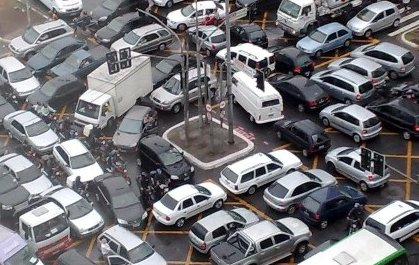
\includegraphics[scale=1]{d.jpg}
\end{center}
\begin{center}

\includegraphics[scale=1]{a.jpg}
\end{center}

\end{document}